\section{587 --- Erect the Fence}
There are some trees, where each tree is represented by $(x,y)$ coordinate in a two-dimensional garden. Your job is to fence the entire garden using the minimum length of rope as it is expensive. The garden is well fenced only if all the trees are enclosed. Your task is to help find the coordinates of trees which are exactly located on the fence perimeter.

\paragraph{Example 1:}

\begin{flushleft}
\textbf{Input}: $[[1,1],[2,2],[2,0],[2,4],[3,3],[4,2]]$

\textbf{Output}: $[[1,1],[2,0],[4,2],[3,3],[2,4]]$

\textbf{Explanation}
\begin{figure}[H]
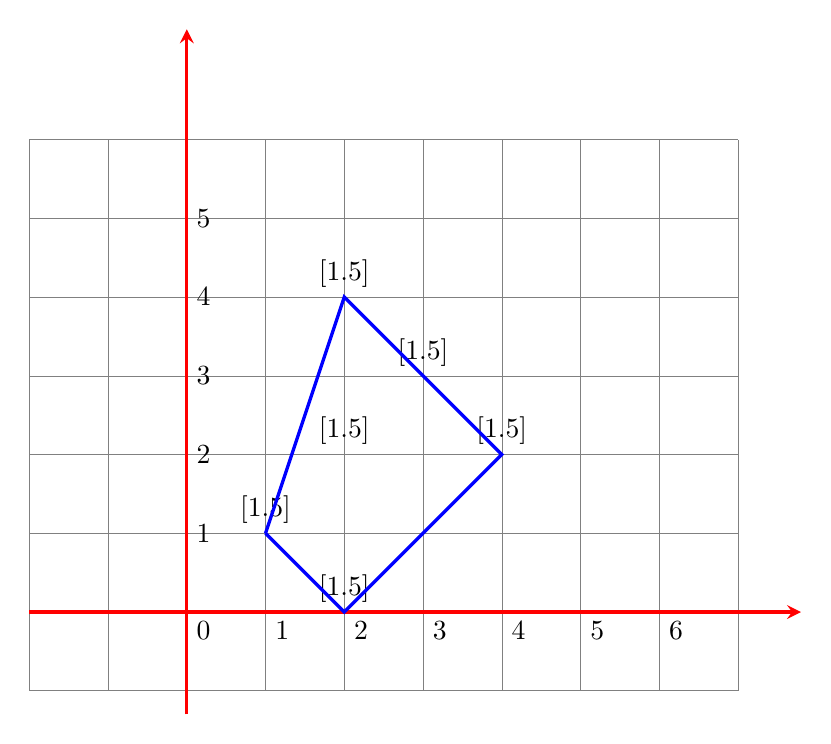
\begin{tikzpicture}
\draw[help lines] (0,0) grid (9,7);
\node at (3,2) [anchor=south] {\Springtree[1.5]};
\node at (4,3) [anchor=south]{\Springtree[1.5]};
\node at (4,1) [anchor=south]{\Springtree[1.5]};
\node at (4,5) [anchor=south]{\Springtree[1.5]};
\node at (5,4) [anchor=south]{\Springtree[1.5]};
\node at (6,3) [anchor=south]{\Springtree[1.5]};
\draw[very thick, >=stealth, ->, red] (0,1) -- (9.8,1);
\draw[very thick, >=stealth, ->, red] (2,-0.3) -- (2,8.4);
\draw[very thick, blue] (3,2) -- (4,1) -- (6,3) -- (5,4) -- (4,5) -- (3,2);
\foreach \x/\y in {2/0,3/1,4/2,5/3,6/4,7/5,8/6}
{\node at (\x, 1) [anchor=north west] {\y};
}
\foreach \x/\y in {2/1,3/2,4/3,5/4,6/5}
{
\node at (2,\x) [anchor=west] {\y};
}

\end{tikzpicture}
\end{figure}
\end{flushleft}

\paragraph{Example 2:}

\begin{flushleft}

\textbf{Input}: $[[1,2],[2,2],[4,2]]$

\textbf{Output}: $[[1,2],[2,2],[4,2]]$

\textbf{Explanation}:

Even you only have trees in a line, you need to use rope to enclose them. 

\begin{figure}[H]
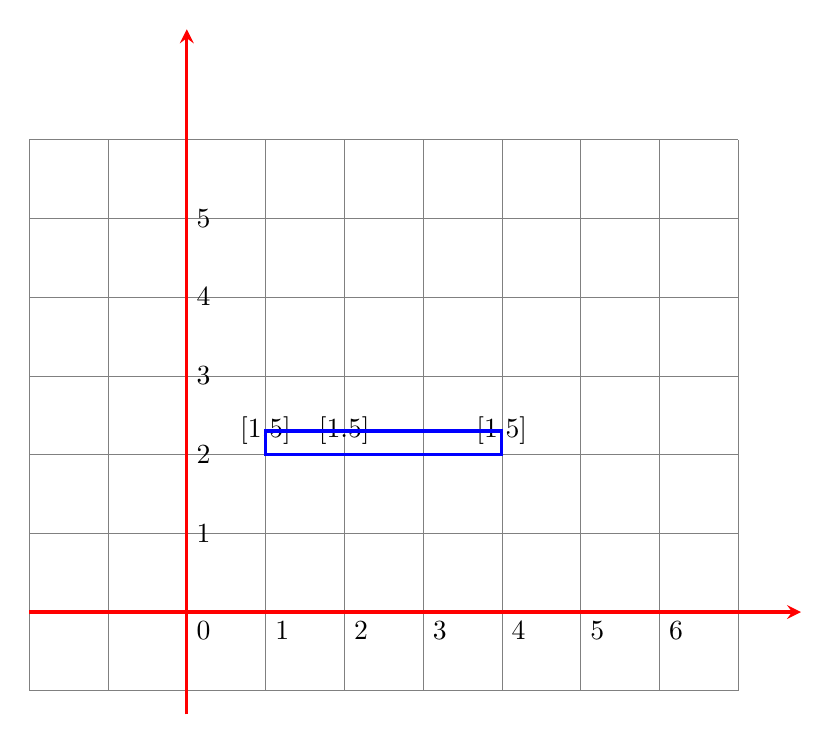
\begin{tikzpicture}
\draw[help lines] (0,0) grid (9,7);
\node at (3,3) [anchor=south] {\Springtree[1.5]};
\node at (4,3) [anchor=south]{\Springtree[1.5]};
\node at (6,3) [anchor=south]{\Springtree[1.5]};
\draw[very thick, >=stealth, ->, red] (0,1) -- (9.8,1);
\draw[very thick, >=stealth, ->, red] (2,-0.3) -- (2,8.4);
\draw[very thick, blue] (3,3) rectangle ++(3, 0.3);
\foreach \x/\y in {2/0,3/1,4/2,5/3,6/4,7/5,8/6}
{\node at (\x, 1) [anchor=north west] {\y};
}
\foreach \x/\y in {2/1,3/2,4/3,5/4,6/5}
{
\node at (2,\x) [anchor=west] {\y};
}

\end{tikzpicture}
\end{figure} 

\end{flushleft}

\paragraph{Note:}

\begin{itemize}
\item All trees should be enclosed together. You cannot cut the rope to enclose trees that will separate them in more than one group.
\item All input integers will range from 0 to 100.
\item The garden has at least one tree.
\item All coordinates are distinct.
\item Input points have NO order. No order required for output.
\end{itemize}

\subsection{Find Convex Hull}